\documentclass[letterpaper,10pt]{article}
\usepackage[utf8]{inputenc}

\usepackage{graphicx}
\usepackage{caption}
\usepackage{subcaption}
\usepackage{amsmath}
\usepackage{listings}
\usepackage[top=1in,bottom=1in,left=1in,right=1in]{geometry}

%opening
\title{Assignment 01 Report}
\author{Luke Fraser}

\begin{document}

\maketitle

\begin{abstract}
In this assignment we were tasked with implementing several image processing tools: Image Sampling, Image Quantization, Histogram Equalization, and Histogram Specification. These tools provide an introduction into image manipulation. Many of the techniques implemented in these exercises will provide useful image adaptations for other projects in the future.
\end{abstract}

\section{Introduction}
Each of the four exercises will be contained in its own section. Each section will review the material as well as the method implemented for each image processing technique. Results will be displayed as images to help aid in the review of each method.

\section{Image Sampling}
\begin{figure}[hbtp]
  \centering
  \begin{subfigure}{4cm}
    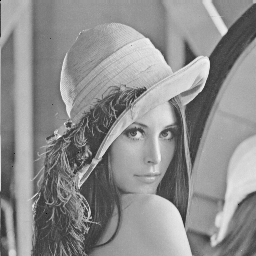
\includegraphics[width=4cm]{images/lenna.png}
    \caption{Original: 256x256.}
  \end{subfigure}
  \begin{subfigure}{4cm}
    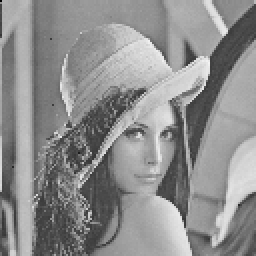
\includegraphics[width=4cm]{images/lenna_subsample128.png}
    \caption{Half: 128x128.}
  \end{subfigure}
  \begin{subfigure}{4cm}
    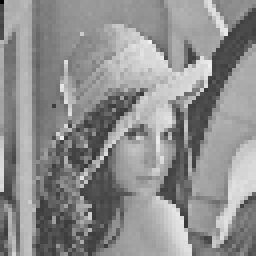
\includegraphics[width=4cm]{images/lenna_subsample64.png}
    \caption{Quarter: 64x64.}
  \end{subfigure}
  \begin{subfigure}{4cm}
    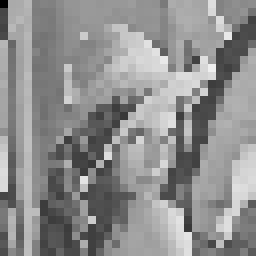
\includegraphics[width=4cm]{images/lenna_subsample32.png}
    \caption{Eighth: 32x32.}
  \end{subfigure}
  \caption{Image Sampling at multiple levels: lenna.pgm.}
  \label{fig:samplelenna}
\end{figure}
\begin{figure}[hbtp]
  \centering
  \begin{subfigure}{4cm}
    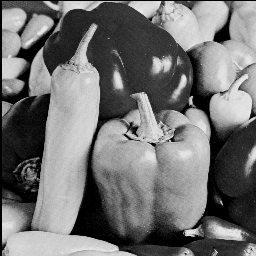
\includegraphics[width=4cm]{images/peppers.png}
    \caption{Original: 256x256.}
  \end{subfigure}
  \begin{subfigure}{4cm}
    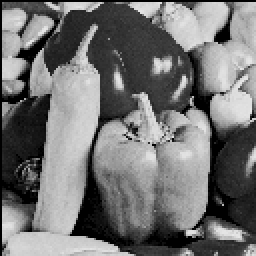
\includegraphics[width=4cm]{images/peppers_subsample128.png}
    \caption{Half: 128x128.}
  \end{subfigure}
  \begin{subfigure}{4cm}
    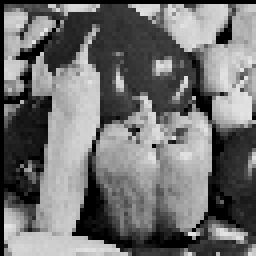
\includegraphics[width=4cm]{images/peppers_subsample64.png}
    \caption{Quarter: 64x64.}
  \end{subfigure}
  \begin{subfigure}{4cm}
    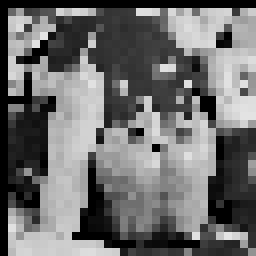
\includegraphics[width=4cm]{images/peppers_subsample32.png}
    \caption{Eighth: 32x32.}
  \end{subfigure}
  \caption{Image Sampling at multiple levels: peppers.pgm.}
  \label{fig:samplepeppers}
\end{figure}

Image sampling takes several samples of an image to build a lower or higher resolution image from the original image. Different methods exist for both down sampling as well as up sampling. In the case of this assignment only down sampling was performed. The images in Figures~\ref{fig:samplelenna} \&~\ref{fig:samplepeppers} illustrate the result of down sampling images at different levels. Each level of sampling visually shows the degradation in the image. The method very simple. No attempt at interpolation or averaging is taken into account. The top left most pixel in a given region is the only pixel that contributes to the down sampled image. The example code below provides a general view of the algorithm used to implement image sampling.

\begin{lstlisting}[frame=single, language=c++]
for (int i=0; i<size; ++i) {
  for (int j=0; j<size; ++j) {
    out_image->setPixelVal(i,j,image.getPixelVal(i*sample, j*sample));
  }
}
\end{lstlisting}
\section{Image Quantization}
\begin{figure}[hbtp]
  \centering
  \begin{subfigure}{3cm}
    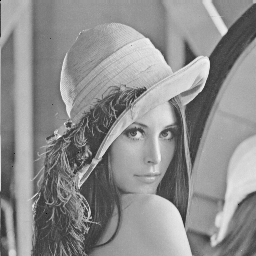
\includegraphics[width=3cm]{images/lenna.png}
    \caption{256 levels}
  \end{subfigure}
  \begin{subfigure}{3cm}
    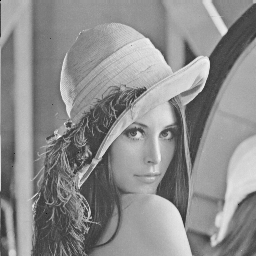
\includegraphics[width=3cm]{images/lenna_quantization128.png}
    \caption{128 levels}
  \end{subfigure}
  \begin{subfigure}{3cm}
    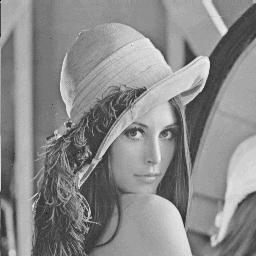
\includegraphics[width=3cm]{images/lenna_quantization32.png}
    \caption{32 levels}
  \end{subfigure}
  \begin{subfigure}{3cm}
    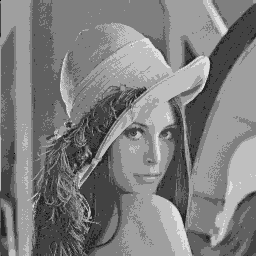
\includegraphics[width=3cm]{images/lenna_quantization8.png}
    \caption{8 levels}
  \end{subfigure}
  \begin{subfigure}{3cm}
    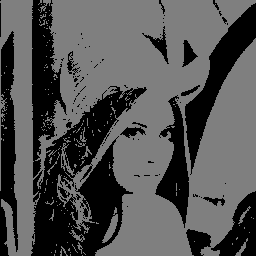
\includegraphics[width=3cm]{images/lenna_quantization2.png}
    \caption{2 levels}
  \end{subfigure}
  \caption{Image Quantization at multiple levels: lenna.pgm.}
  \label{fig:quantlenna}
\end{figure}
\begin{figure}[hbtp]
  \centering
  \begin{subfigure}{3cm}
    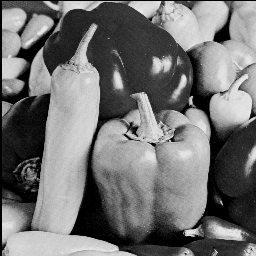
\includegraphics[width=3cm]{images/peppers.png}
    \caption{256 levels}
  \end{subfigure}
  \begin{subfigure}{3cm}
    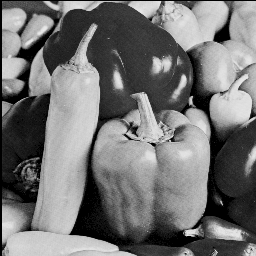
\includegraphics[width=3cm]{images/peppers_quantization128.png}
    \caption{128 levels}
  \end{subfigure}
  \begin{subfigure}{3cm}
    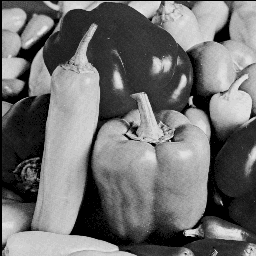
\includegraphics[width=3cm]{images/peppers_quantization32.png}
    \caption{32 levels}
  \end{subfigure}
  \begin{subfigure}{3cm}
    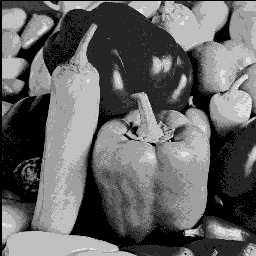
\includegraphics[width=3cm]{images/peppers_quantization8.png}
    \caption{8 levels}
  \end{subfigure}
  \begin{subfigure}{3cm}
    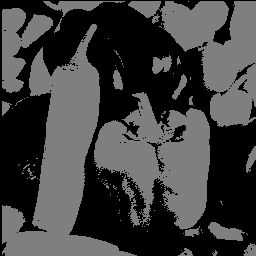
\includegraphics[width=3cm]{images/peppers_quantization2.png}
    \caption{2 levels}
  \end{subfigure}
  \caption{Image Quantization at multiple levels: peppers.pgm.}
  \label{fig:quantlenna}
\end{figure}
Image quantization is a very useful image processing operation. It can be used in image compression, segmentation, and as an artistic style. The use of quantization can help remove unnecessary information from an image in order to shrink file size. The human eye in many cases isn't sensitive enough to notice major changes in different quantization levels. It is only at the low end of quantization that its effects are quite apparent. The method implemented for this exercise is very simple. The method takes advantage of c++ integer rounding operations. First division is performed followed by multiplication. Integer division followed by multiplication is a lossy operation in c++. for example 4/2=2, but 3/2=1 with integer division. This provides an easy method to quantize data. The example code below illustrates the method further.
\begin{lstlisting}[frame=single, language=c++]
for (int i=0; i<rows; ++i) {
  for (int j=0; j<cols; ++j) {
    out_image->setPixelVal(i,j,(256/type)*(image.getPixelVal(i,j)/(256/type)));
  }
}
\end{lstlisting}
\section{Histogram Equalization}
\begin{figure}[hbtp]
  \centering
  \begin{subfigure}{4cm}
    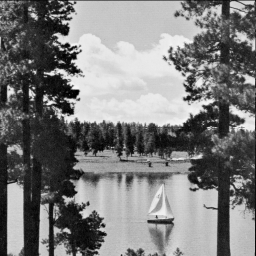
\includegraphics[width=4cm]{images/boat.png}
    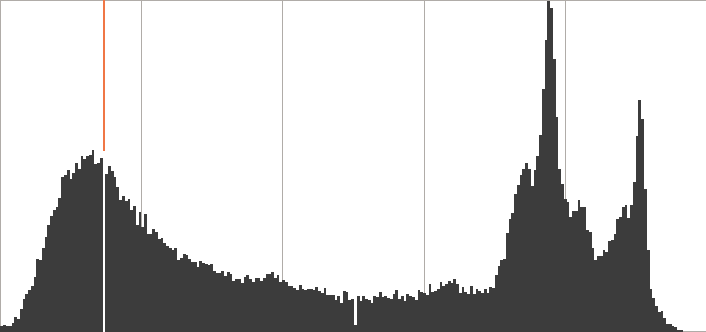
\includegraphics[width=4cm]{images/boat_hist.png}
    \caption{original}
  \end{subfigure}
  \begin{subfigure}{4cm}
    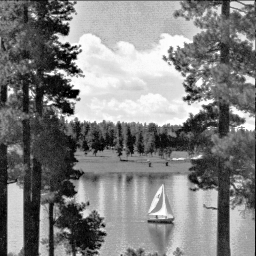
\includegraphics[width=4cm]{images/boat_equalization.png}
    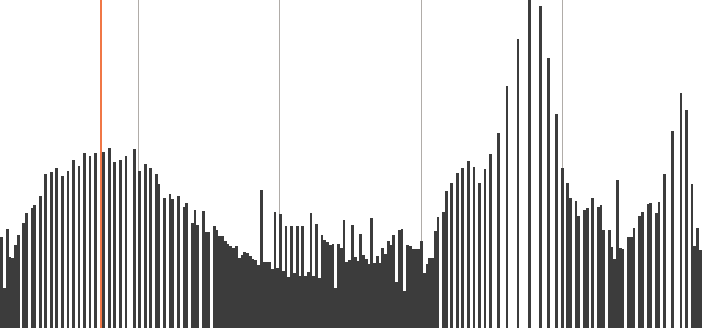
\includegraphics[width=4cm]{images/boat_equalization_hist.png}
    \caption{equalization}
  \end{subfigure}
  \begin{subfigure}{4cm}
    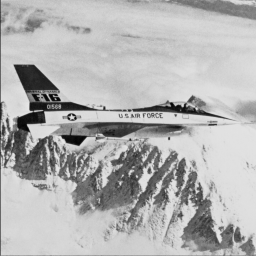
\includegraphics[width=4cm]{images/f_16.png}
    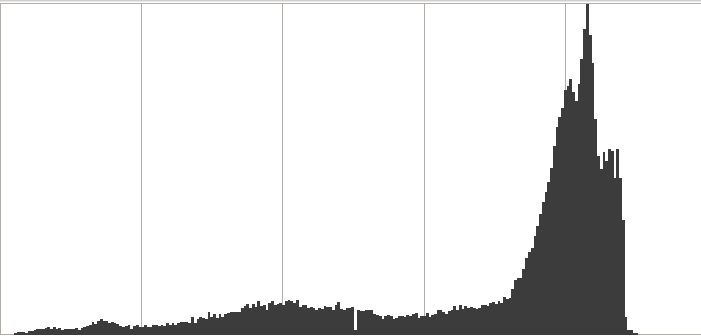
\includegraphics[width=4cm]{images/f_16_hist.png}
    \caption{original}
  \end{subfigure}
  \begin{subfigure}{4cm}
    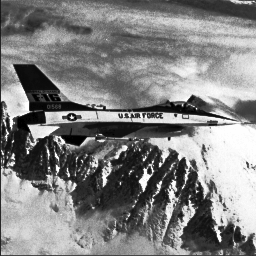
\includegraphics[width=4cm]{images/f_16_equalization.png}
    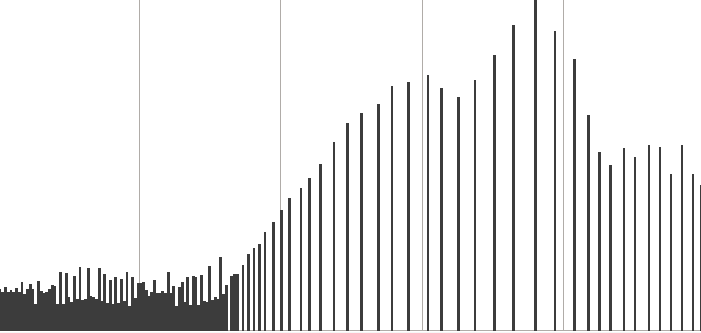
\includegraphics[width=4cm]{images/f_16_equalization_hist.png}
    \caption{equalization}
  \end{subfigure}
  \caption{Histogram Equalization}
  \label{fig:equalization}
\end{figure}
Histogram equalization is a useful technique to level off an images histogram. The effects of histogram equalization can be very apparent. Low contrast portions of the image can present new detail after performing histogram equalization. The method is quite simple to perform and positive results can be seen quickly. The algorithm implemented for this exercise first finds the normalized histogram of the image which represents the PDF of the image. The cumulative density function is then found and ultimately used for the equalization transformation. A map is generated that maps each pixel value to its corresponding equalized form. This map is then used to build the result image. The example code below illustrates the procedure. The images in Figure~\ref{fig:equalization} show both before and after images of the process as well as the images corresponding histograms.

\begin{lstlisting}[frame=single, language=c++]
float * in_hist = img_tools::ImHist(in_image);

float * in_cum_hist = img_tools::ImCumHist(in_hist);

int map[256];
for (int i=0; i<256; ++i) {
  map[i] = in_cum_hist[i] * 255;
}
ImageType * mapped_image = img_tools::MapImage(map, in_image);
\end{lstlisting}
\section{Histogram Specification}
\begin{figure}[hbtp]
  \centering
  \begin{subfigure}{4cm}
    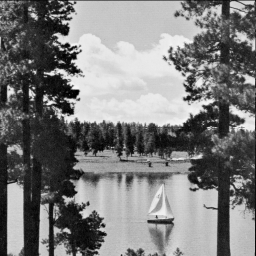
\includegraphics[width=4cm]{images/boat.png}
    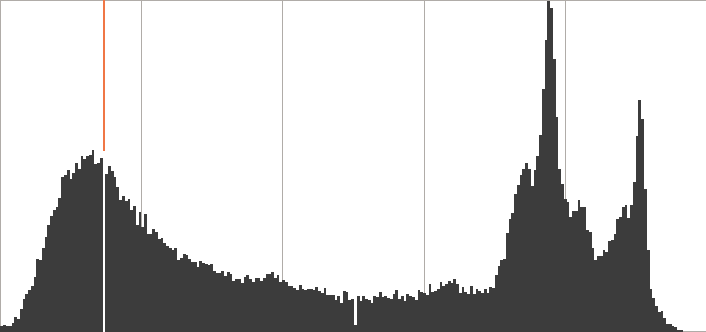
\includegraphics[width=4cm]{images/boat_hist.png}
    \caption{original}
  \end{subfigure}
  \begin{subfigure}{4cm}
    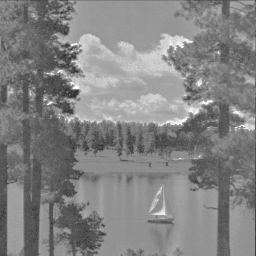
\includegraphics[width=4cm]{images/boat_specification.png}
    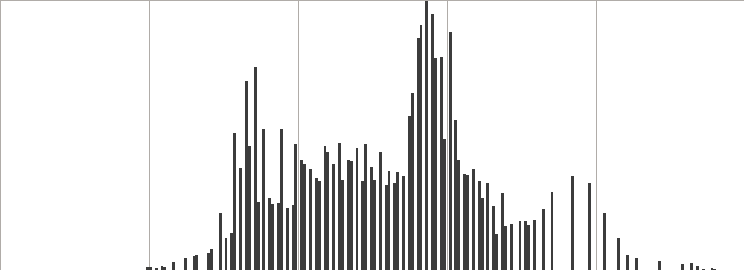
\includegraphics[width=4cm]{images/boat_specification_hist.png}
    \caption{specification}
  \end{subfigure}
  \begin{subfigure}{4cm}
    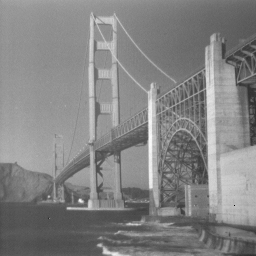
\includegraphics[width=4cm]{images/sf.png}
    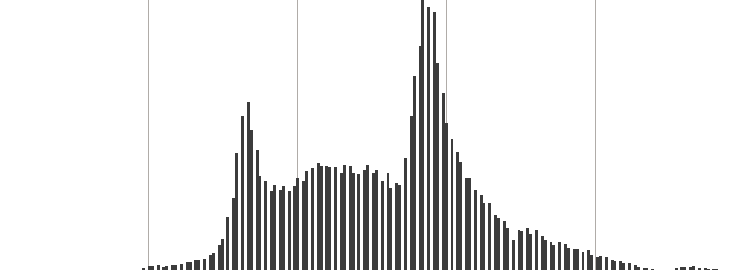
\includegraphics[width=4cm]{images/sf_hist.png}
    \caption{target hist}
  \end{subfigure}
  \caption{Histogram Specification is used to match the histogram of the boat with the sf image.}
  \label{fig:specificationboat}
\end{figure}
\begin{figure}[hbtp]
  \centering
  \begin{subfigure}{4cm}
    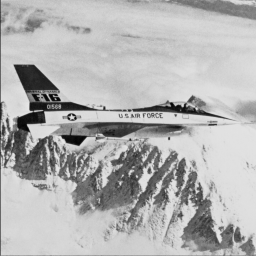
\includegraphics[width=4cm]{images/f_16.png}
    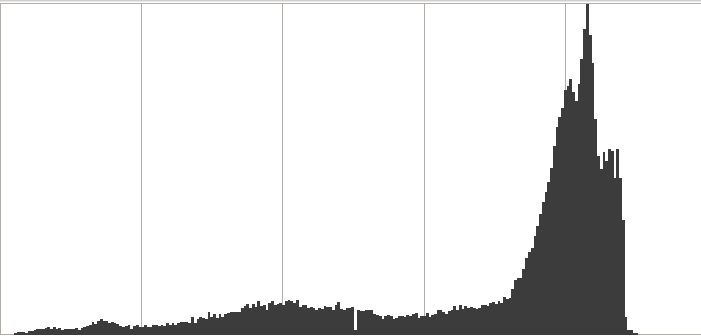
\includegraphics[width=4cm]{images/f_16_hist.png}
    \caption{original}
  \end{subfigure}
  \begin{subfigure}{4cm}
    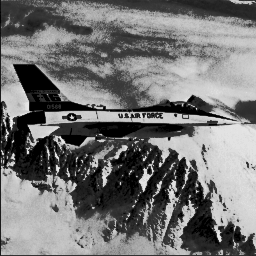
\includegraphics[width=4cm]{images/f_16_specification.png}
    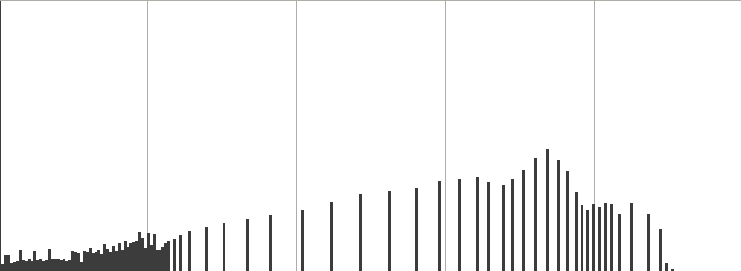
\includegraphics[width=4cm]{images/f_16_specification_hist.png}
    \caption{specification}
  \end{subfigure}
  \begin{subfigure}{4cm}
    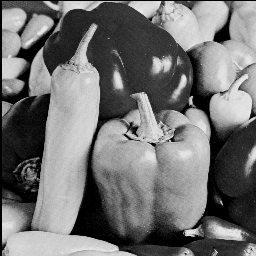
\includegraphics[width=4cm]{images/peppers.png}
    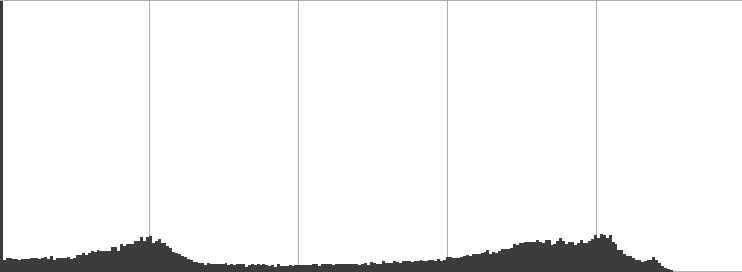
\includegraphics[width=4cm]{images/peppers_hist.png}
    \caption{target hist}
  \end{subfigure}
  \caption{Histogram Specification is used to match the histogram of the f 16 with the peppers image.}
  \label{fig:specificationf}
\end{figure}
Histogram specification takes histogram equalization one step further. Instead of simply equalizing a histogram over the levels of an image, specification transforms an image with a given histogram to another specified histogram. In the case of this exercise an image is transformed into the histogram of another image. The implementation works quite well as can be seen in the results. The method is similar to equalization however an extra step of inverse equalization transformation is performed on the input image to map it into the supplied images histogram. Figures~\ref{fig:specificationboat} \&~\ref{fig:specificationf} show the results of the algorithm. Example code is also shown below outlining the algorithm and its implementation.
\\ \\ \\ \\
\begin{lstlisting}[frame=single, language=c++]
float * in_hist = img_tools::ImHist(in_image);
float * out_hist = img_tools::ImHist(out_image);

float * in_cum_hist = img_tools::ImCumHist(in_hist);
float * out_cum_hist = img_tools::ImCumHist(out_hist);

int * map = img_tools::InverseMap(in_cum_hist, out_cum_hist);

ImageType * mapped_image = img_tools::MapImage(map, in_image);
\end{lstlisting}
\end{document}
